\section{Rezolvarea numerică a ecuațiilor algebrice prin metoda coardei.}

În analiză numerică, \textbf{metoda coardei} (sau \textit{metoda falsei poziții}, \textit{metoda falsi}) 
este o metodă de determinare a rădăcinii unei funcții pe un interval. \par

Metoda bisecției, cu toată simplitatea ei nu este efectivă în cazurile când rezultatul
trebuie obținut prin un număr mic de iterații, cu o exactitate înaltă, segmentul inițial care
conține soluția fiind destul de mare. În acest caz este mai potrivită divizarea segmentului în
părți proporționale, proporția fiind dată de punctul de intersecție al coardei care uneşte
extremitățile segmentului cu axa $O_x$.

\begin{figure}[H]0
    \centering
    \includestandalone{assets/regula-falsi-plot}
    \caption{Demonstrarea grafică a metodei coardei.}
    \label{fig:regula-falsi-figure}
\end{figure}

La fel ca metoda înjumătățirii intervalului, metoda falsei poziții începe 
cu două puncte $a$ și $b$ astfel încât $f(a)$ și $f(b)$ sunt de semne opuse, 
ceea ce înseamnă, conform teoremei valorilor intermediare că funcția 
continuă $f$ are cel puțin un zero în intervalul $[a, b]$. \par

\begin{figure}[H]
    \centering
    \includestandalone[scale=0.8]{assets/regula-falsi-flowchart}
    \caption{Diagrama metodei coardei.}
    \label{fig:regula-falsi-flowchart}
\end{figure}

\lstinputlisting[language={[Sharp]C}]{assets/listings/RegulaFalsi.cs} \par

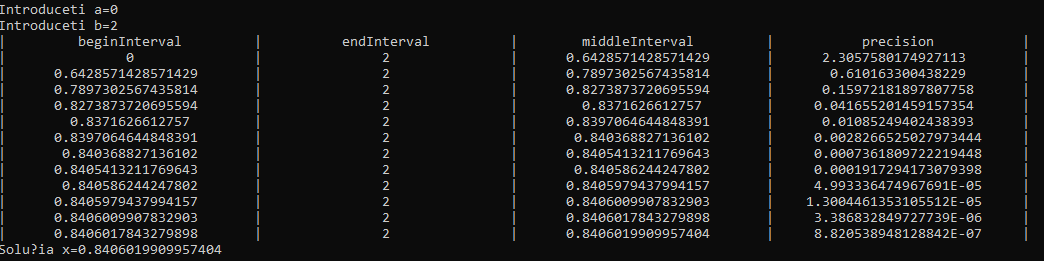
\includegraphics[width=0.9\textwidth]{assets/listings/regula-falsi-output.png} \par

\clearpage
